% --------------------------------------------------------------------------------------------------
\section{Modelling}
In order to model and forecast the electricity comsumption, several methods have been applied. 
Due to the high frequency of seasonality of the dataset, Holt-Winters method (exponential smoothing) 
did not provide suitable results. Similarly, Random Forest algorithm modelling did show very high 
computational time. Models using Random Forest algorithm were not investigated further and will not 
be discussed in this report. R-code for this algothm and everthing presented in this report are 
available in the attached R script files.\\

This report will present models and forecasts using SARIMA, Neural Network and XGBoost methods 
computed with or without covariate dataset.

% --------------------------------------------------------------------------------------------------
\subsection{Dataset splitting}

The dataset is split into a training and a testing set. The last period of Electricity power is 
taken as the testing test while the rest of the dataset is the training set. R-software code is 
presented in listing \ref{lst_split} below and datasets are presented in figure 
\ref{figure_train_test_set}. 

\begin{lstlisting}[language=R, caption={Dataset splitting into train/test sets}, captionpos=b, label={lst_split}]
# Split in train/test set
v <- ts(data[,1:3], start=c(2010,1), frequency=96)
v_start <- start(v)
v_end   <- end(v)

# remove 2 last periods for training set:
v_train <- window(v, start=v_start , end=c(v_end[1],v_end[2]-2*96))
# start after 2 to last period for testing set:
v_test  <- window(v, start=c(v_end[1], v_end[2]-2*96+1), end=v_end)
\end{lstlisting}

\begin{figure}[H]
\centering
 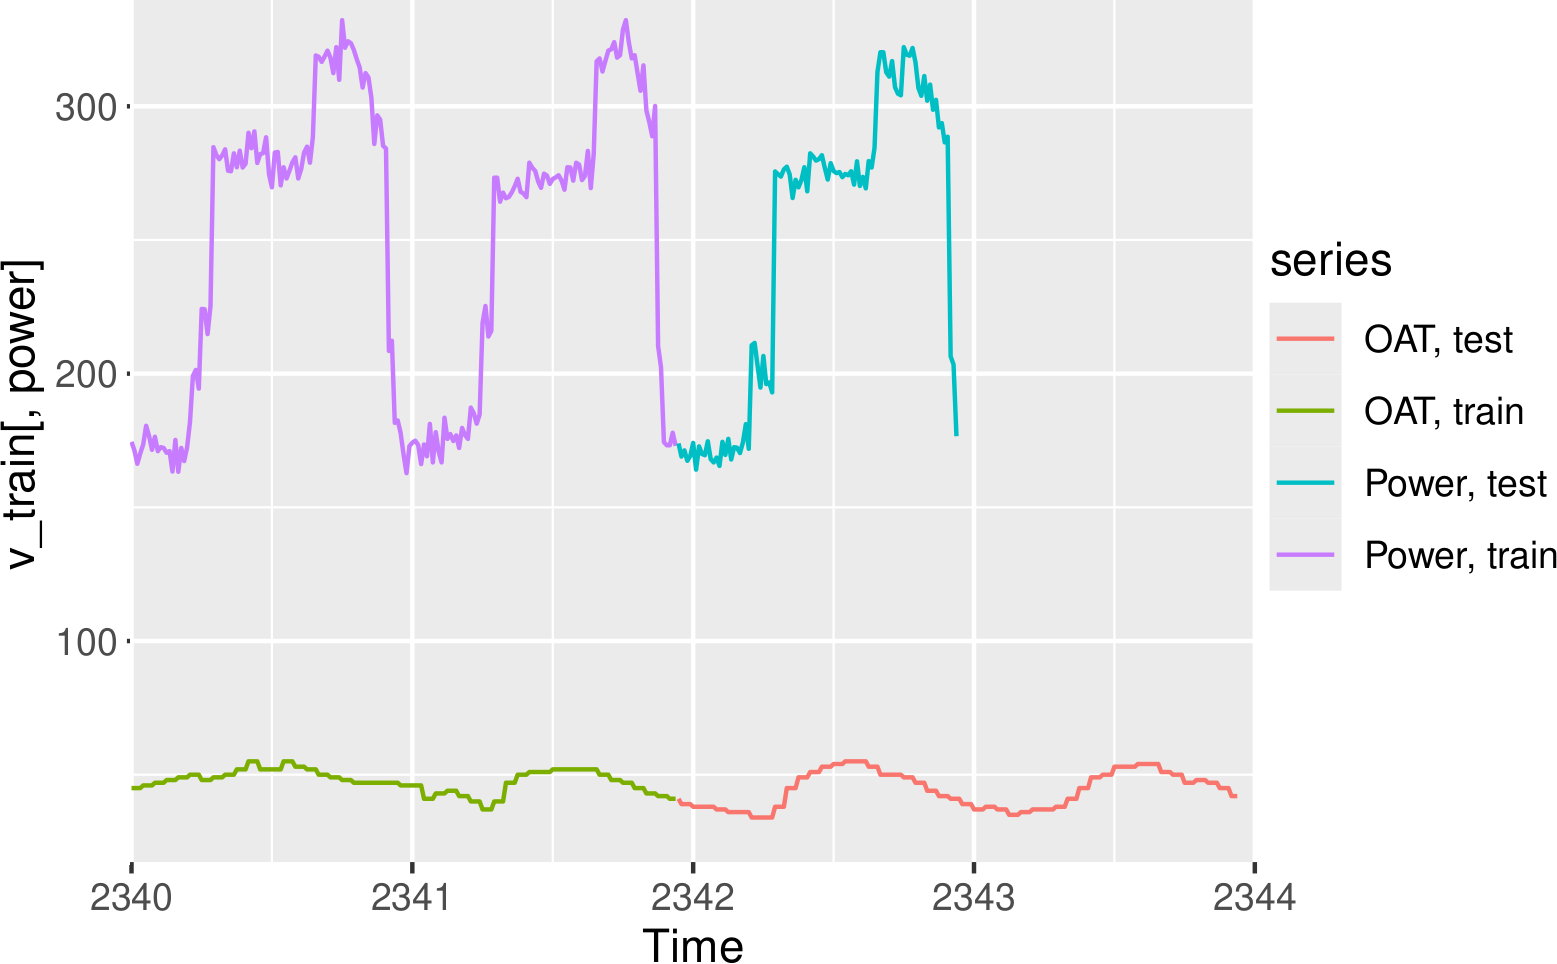
\includegraphics[scale=0.65]{figures/train_test_set.png}
\caption{Training and testing sets of the variables Power and OAT (Outer Air Temperature).}
\label{figure_train_test_set}
\end{figure}


% --------------------------------------------------------------------------------------------------
\subsection{SARIMA}
Figure \ref{figure_decompose} shows high seasonality in the dataset therefore ARIMA methodology 
would not be appropriate for this study. Seasonality ARIMA (SARIMA) method is applied. Due to the 
relatively long computation time (more than one hour per computation), grid-seach is not implemented 
to search for the best parameters. See listing \ref{lst_sarima} for R-code. Figures 
\ref{figure_residuals_sarima} and \ref{figure_fit_sarima} presents the best SARIMA model with 
prediction for fitting with and without considering the OAT covariate.

Table \ref{table_sarima} shows few statistics of the models and show little improvement in the 
fitting when considering OAT covariates.

\begin{table}[H]
\centering \begin{tabular}{c|cc}
                 & With OAT covariate & Without OAT covariate\\\hline\hline
RMSE             &  8.31     &  8.60 \\
p-value          & 2.2e$^{-16}$ &  2.2e$^{-16}$ \\
Computation time &  1h10     &  56 min \\
\end{tabular}
\caption{Statistics of SARIMA modelling.}
\label{table_sarima}
\end{table}

Noise residuals of this model (figure \ref{figure_residuals_sarima}, p-values in table 
\ref{table_sarima}) still show significant signals that are not taken into account with this model. 
Increasing the values of the parameters seems to be necessary however, updating the parameters 
led to computational failure.

\begin{figure}[!h]
\centering
 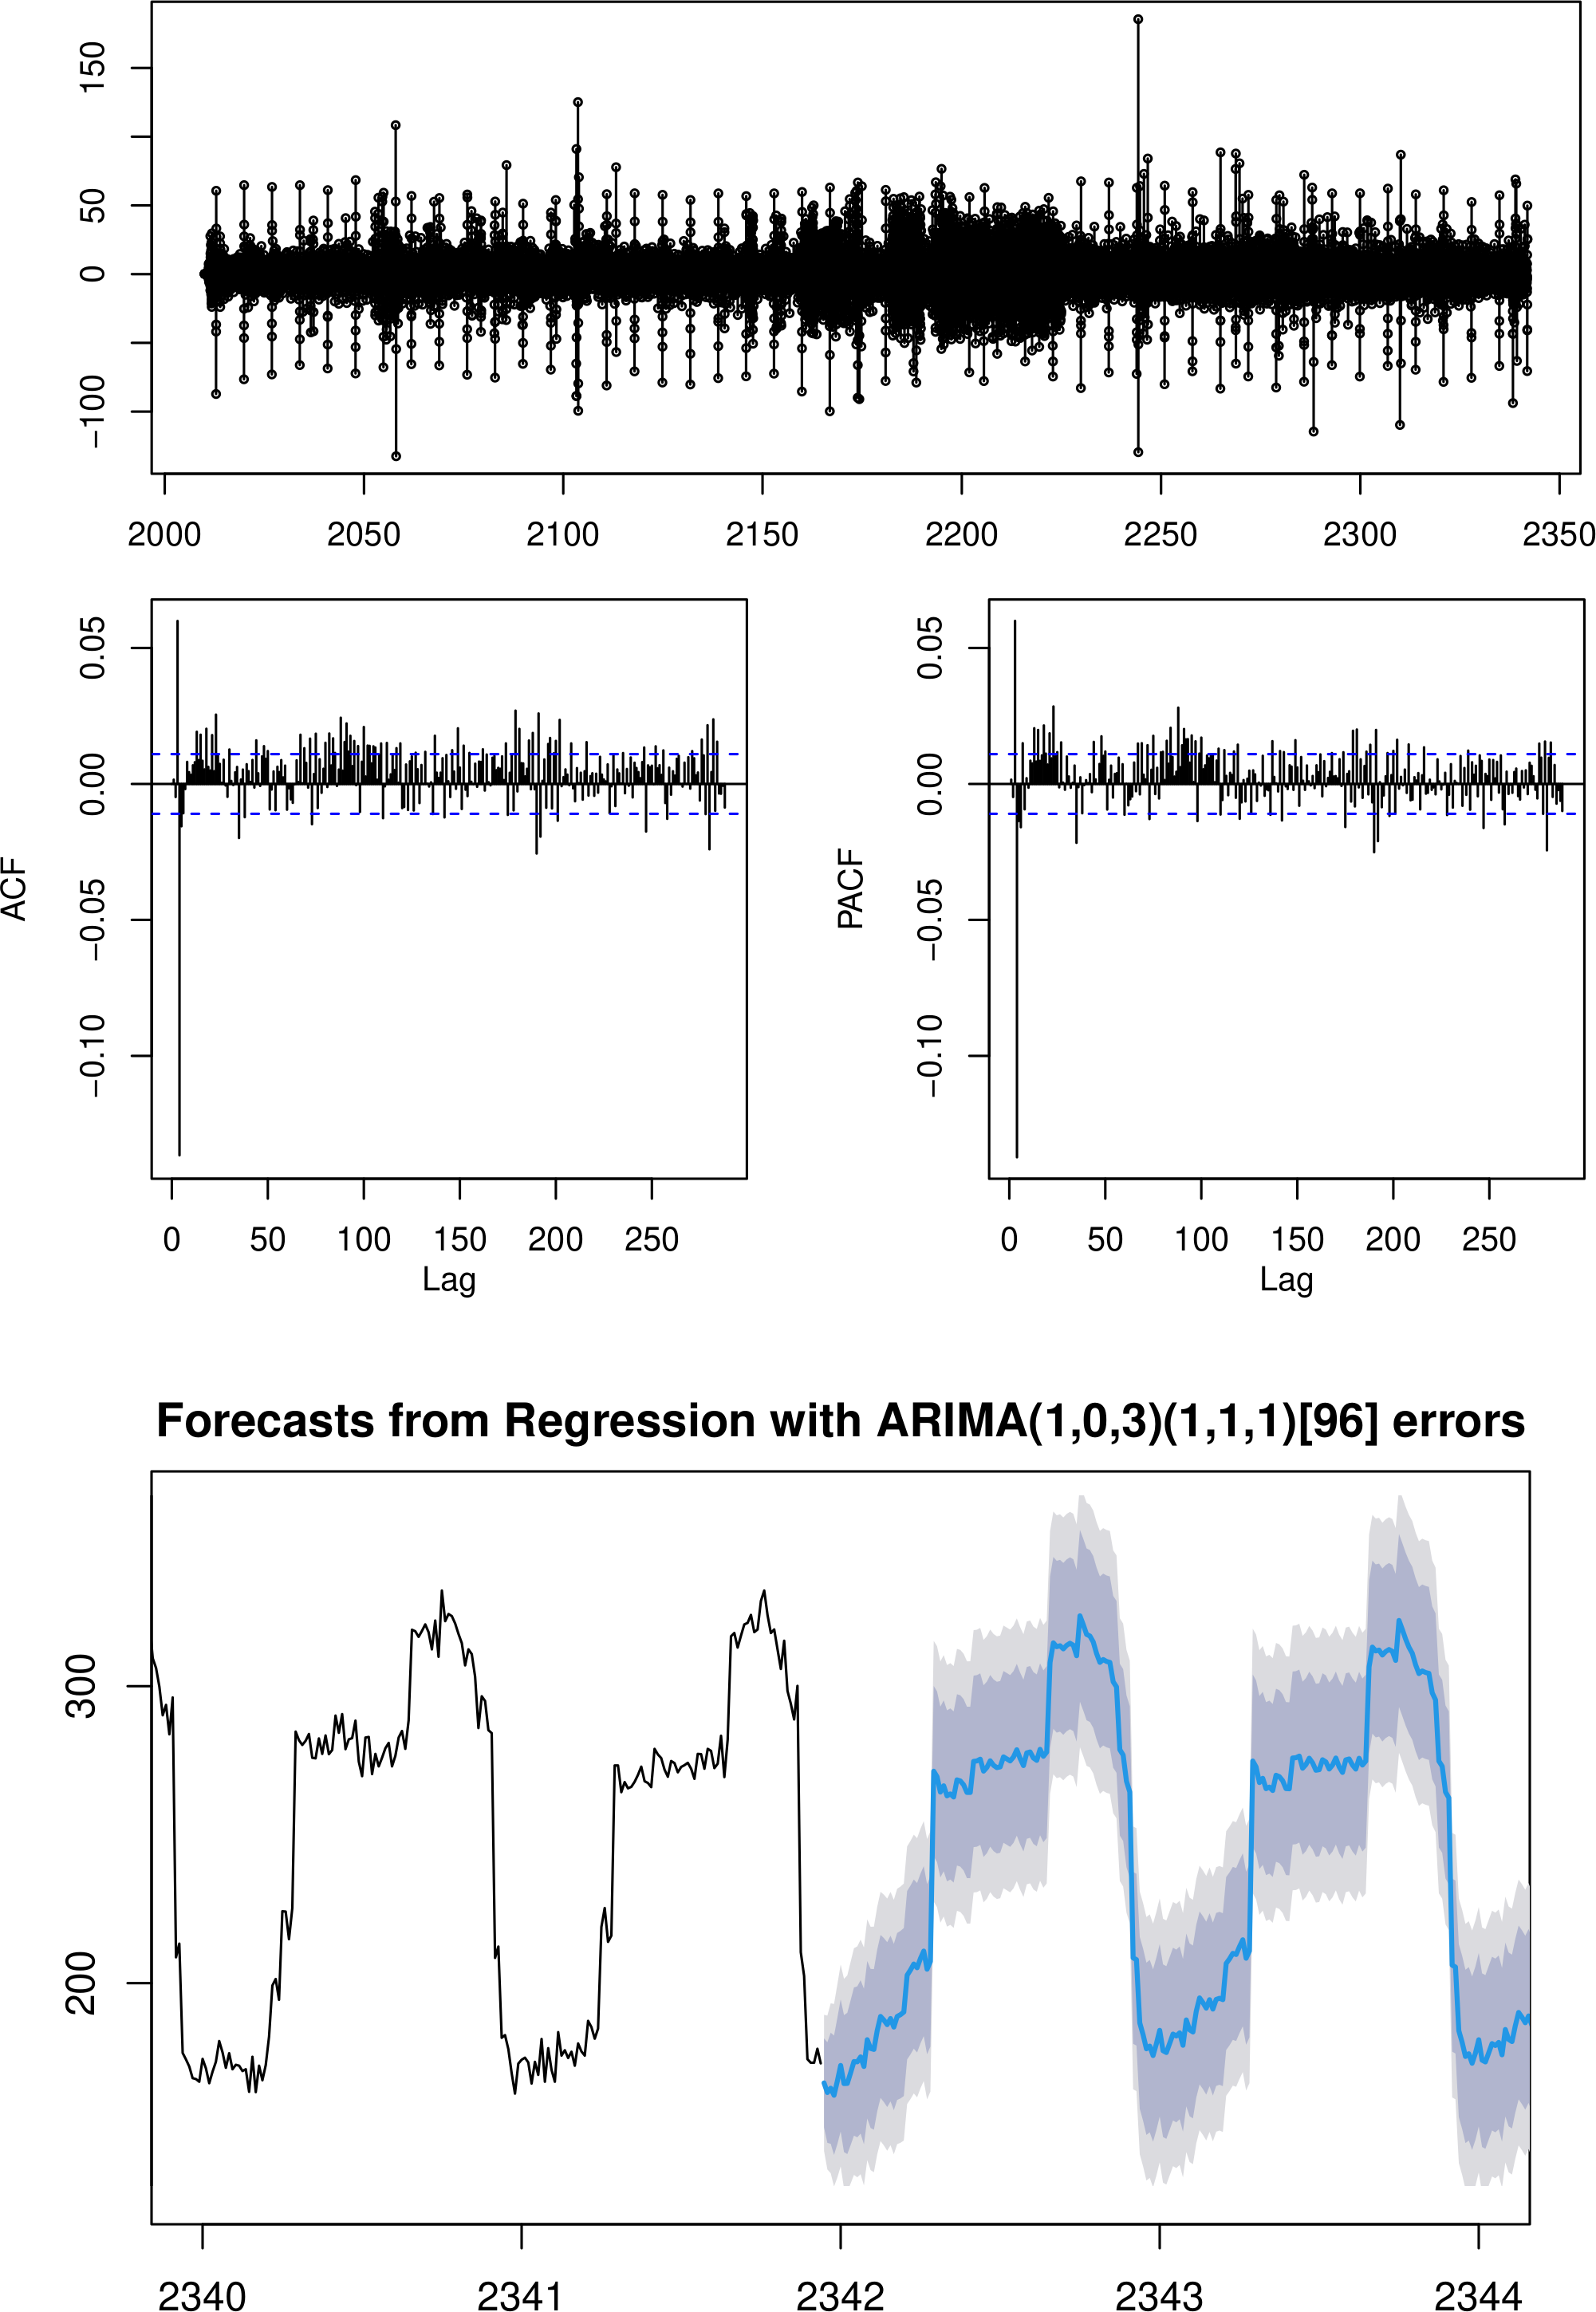
\includegraphics[scale=0.45]{figures/figure_residuals_sarima.png}
 \caption{Modelling and forecasting using SARIMA algorithm with (1,0,3)(1,1,1)[96] parameters and OAT covariates.}
\label{figure_residuals_sarima}
\end{figure}

\begin{figure}[H]
\centering
 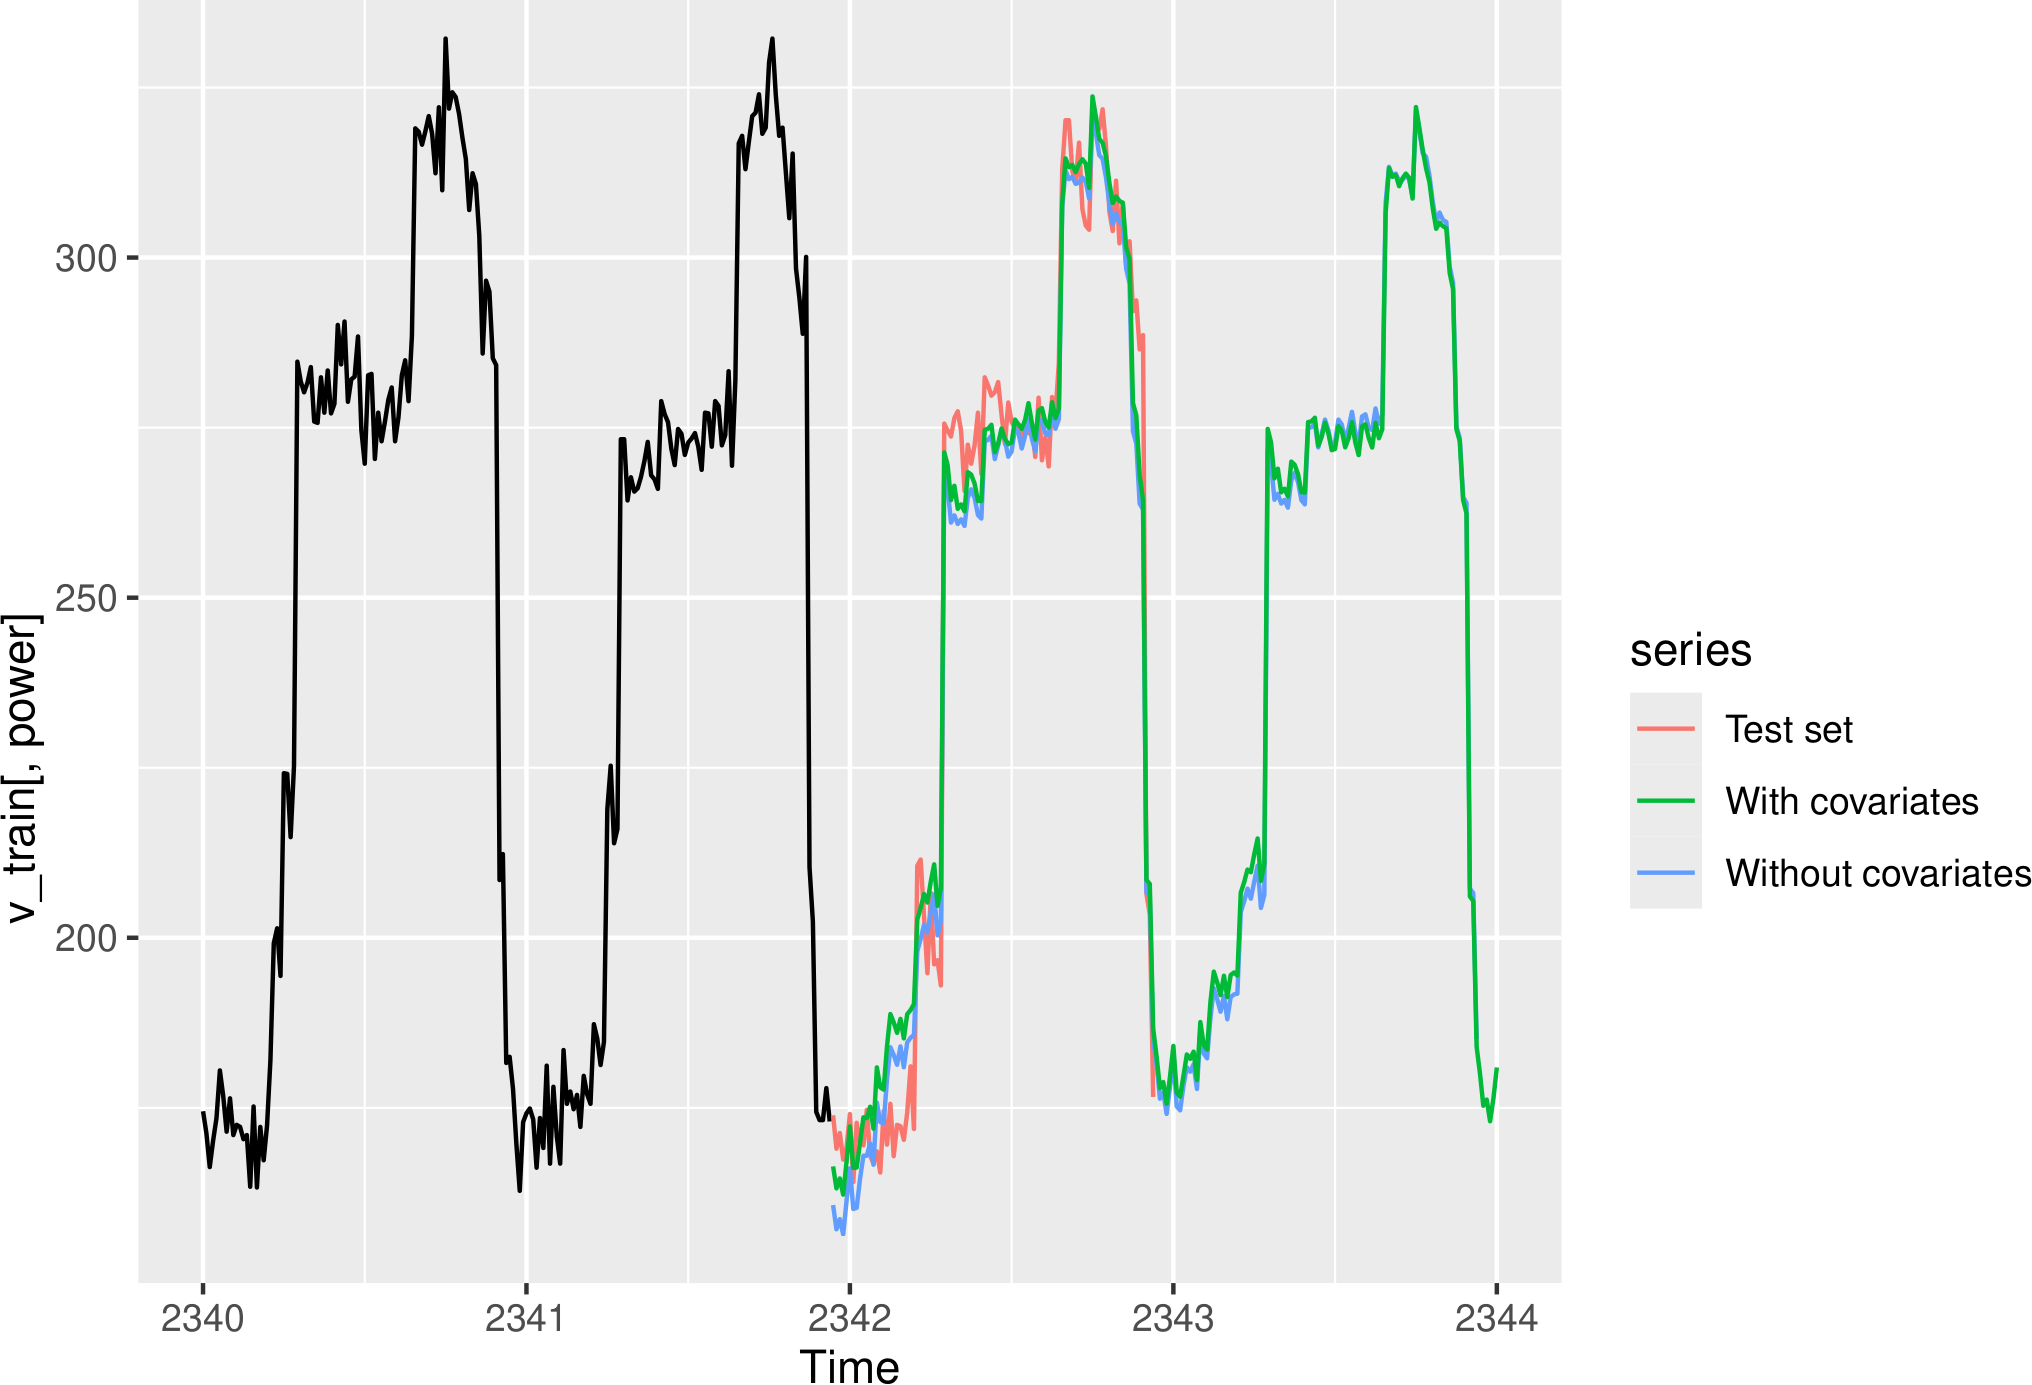
\includegraphics[scale=0.5]{figures/figure_fit_sarima.png}
\caption{Testing set and forecast of the Electricity consumption using SARIMA algorith with 
(1,0,3)(1,1,1)[96] parameters with (green line) and without OAT covariate (blue line).}
\label{figure_fit_sarima}
\end{figure}

\newpage
\begin{lstlisting}[language=R, caption={R code for SARIMA modelling and forecasting}, captionpos=b, label={lst_sarima}]
  if ( covariates )
    {
    start.time <- Sys.time()
    fit = Arima(v_train[,power], xreg=v_train[,oat], order=c(1,0,3), seasonal=c(1,1,1))
    end.time <- Sys.time()
    cat("timing :", (end.time-start.time), "\n")

    checkresiduals(fit)
    tsdisplay(fit$residuals)

    fc <- forecast(fit, xreg=v_train[,oat], h=192)

    rmse = calc_rmse(v_test[,power], fc$mean)
    cat("RMSE SARIMA (with covariates) :", rmse, "\n")
    }
  else
    {
    start.time <- Sys.time()
    fit <- Arima(v_train[,power], order=c(1,0,3), seasonal=c(1,1,1))
    end.time <- Sys.time()
    cat("timing :", (end.time-start.time), "\n")

    checkresiduals(fit)
    tsdisplay(fit$residuals)

    fc <- forecast(fit, h=192)

    rmse = calc_rmse(v_test[,power], fc$mean)
    cat("RMSE SARIMA (without covariates) :", rmse, "\n")
\end{lstlisting}

% --------------------------------------------------------------------------------------------------
\subsection{Neural-Network}
Grid-search analysis is performed to search for the best parameters \textit{i.e.} the set of 
parameters that minimize the root-mean-square-error between the data and the model (see attached R 
script files for complete code). Results show that parameters (7,3,6) are best-suited for Neural 
Network modelling of the Electricity consumption and parameters (4,2,4) are best-suited when 
considering outer-air temperature data as a covariate. Modeling and forecasting using these 
parameters are presented in figures \ref{figure_residuals_NN} and \ref{figure_fit_NN}. Listing 
\ref{lst_NN} presents the piece of R code used to model and forecast the electricity consumption. 

\begin{figure}[H]
\centering
 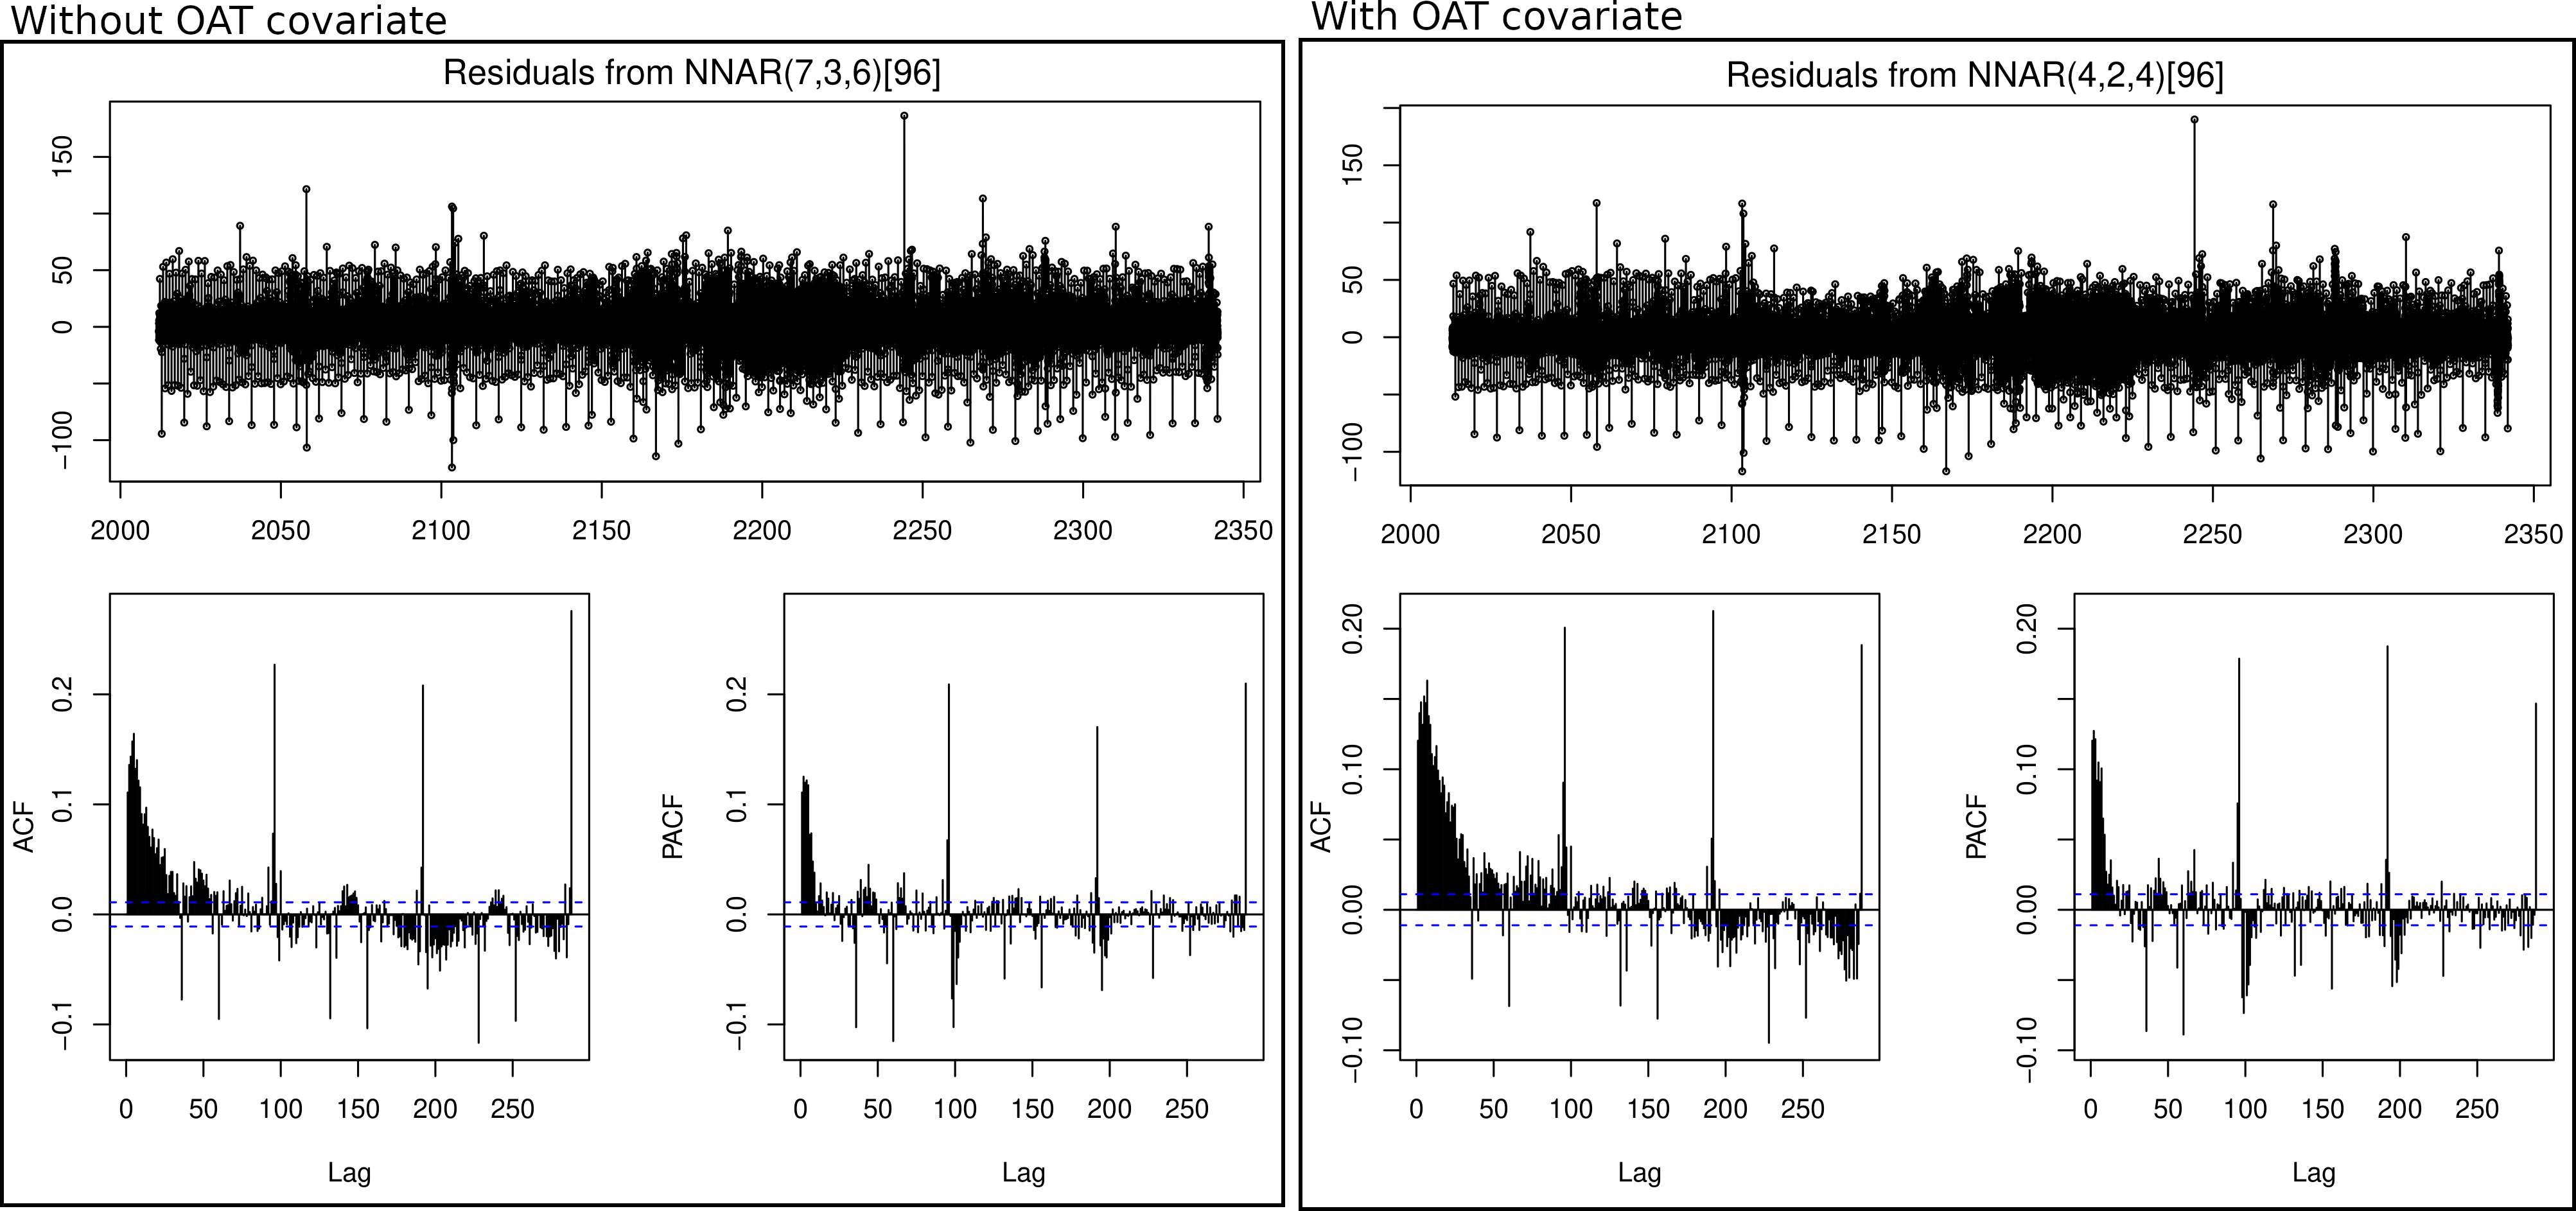
\includegraphics[scale=0.35]{figures/figure_residuals_NN.png}
 \caption{Modelling using Neural Network algorithm with (7,3,6)[96] parameters when not considering OAT covariates and (4,2,4)[96] when considering OAT covariates.}
 \label{figure_residuals_NN}
\end{figure}

\begin{figure}[H]
\centering
 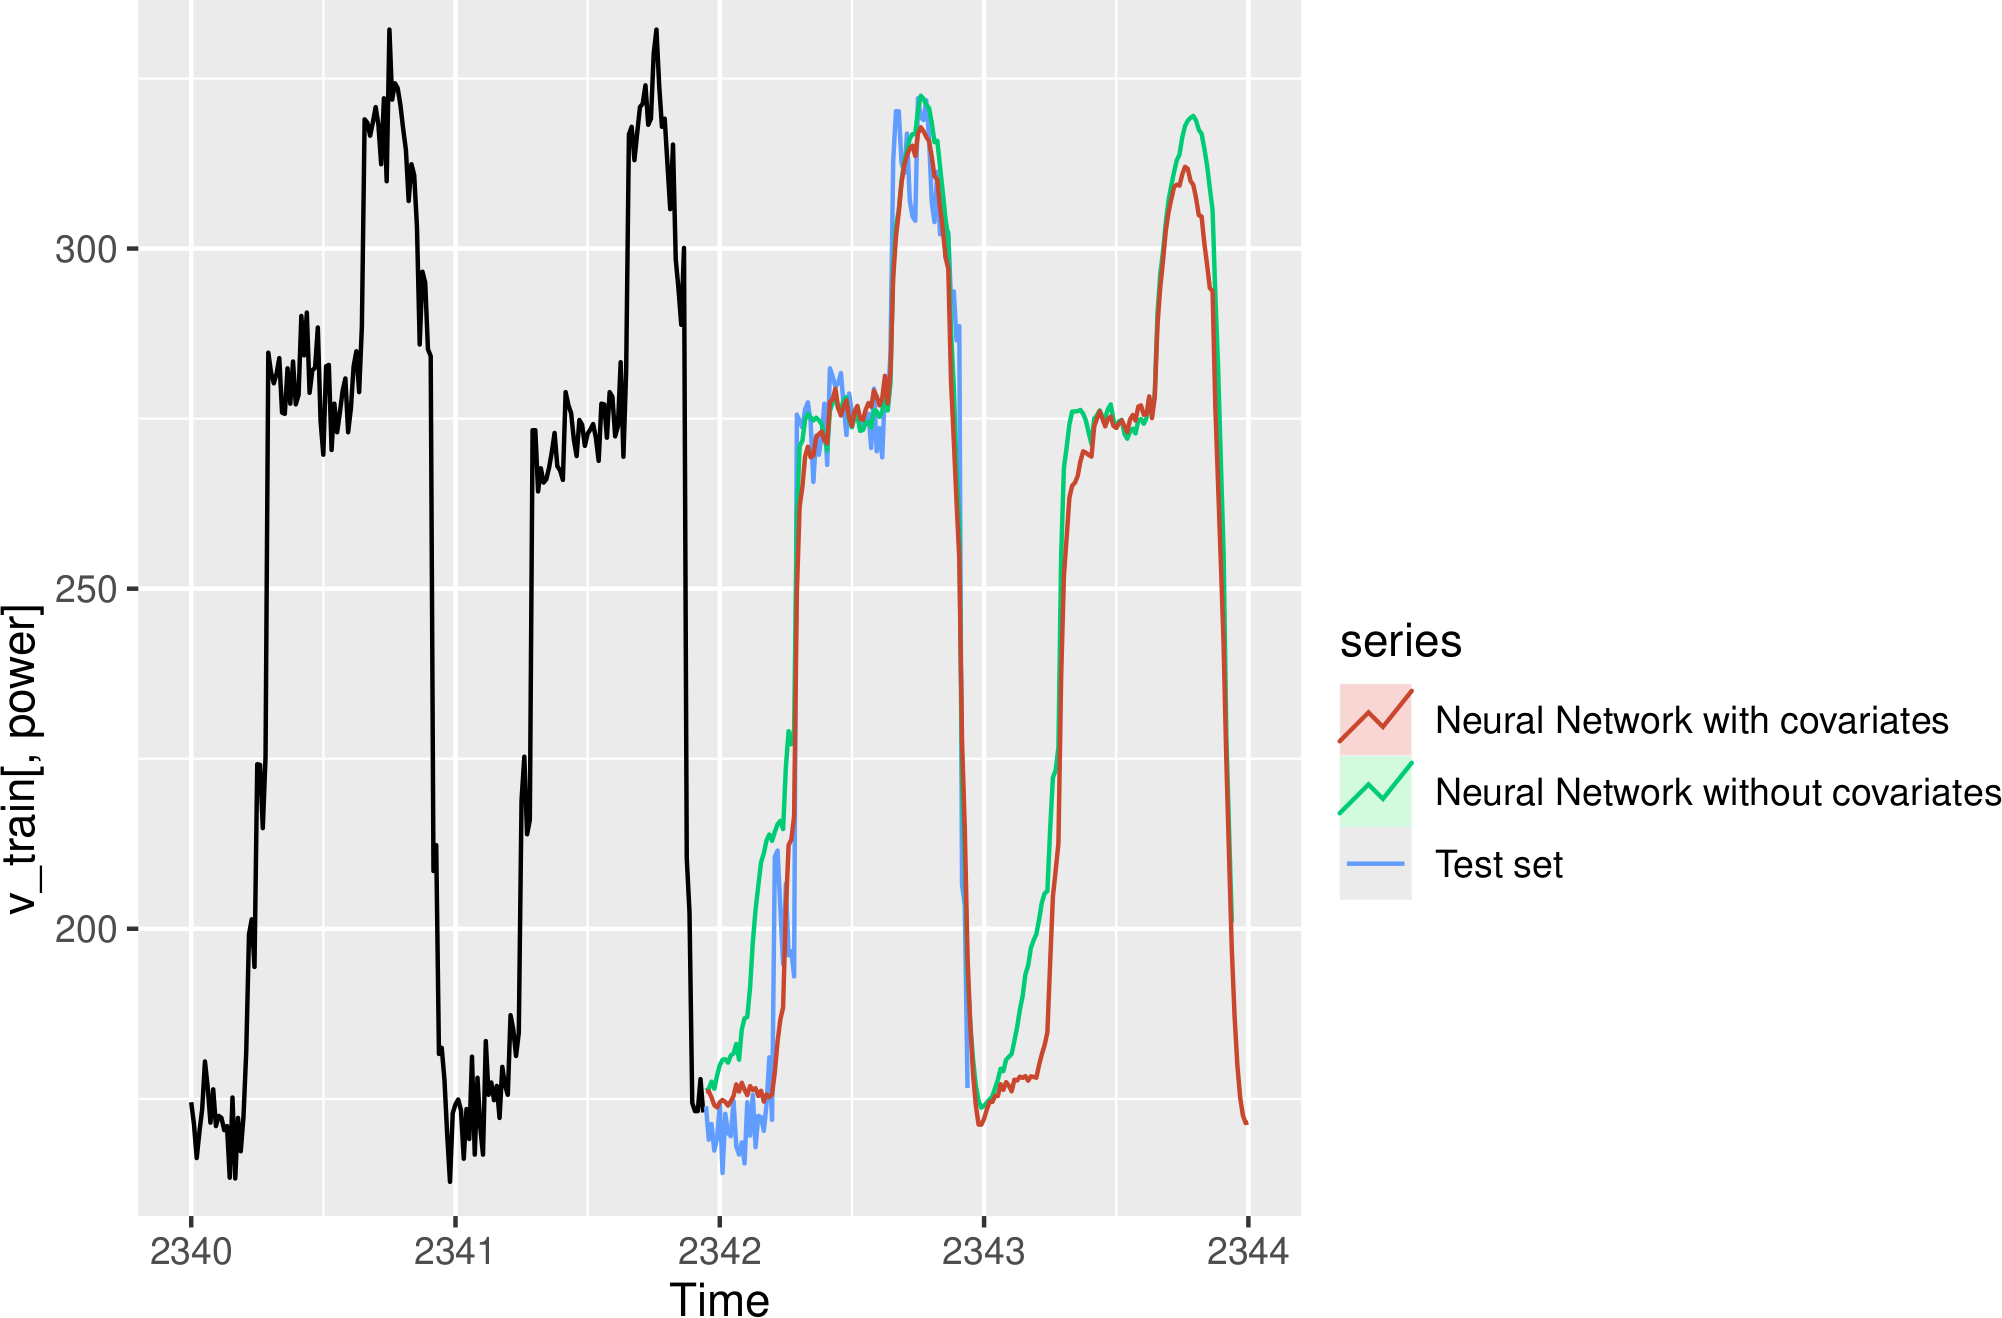
\includegraphics[scale=0.55]{figures/figure_fit_NN.png}
\caption{Testing set (blue line) and forecast of the electricity consumption using Neural Network algorith with (red line) and without OAT covariate (green line).}
\label{figure_fit_NN}
\end{figure}

\begin{lstlisting}[language=R, caption={R code for Neural Network method modelling and forecasting}, captionpos=b, label={lst_NN}]
  if ( covariates )
    {
    start.time <- Sys.time()
    fit  = nnetar(v_train[,power], xreg=v_train[,oat], p=4, P=2)
    end.time <- Sys.time()
    cat("timing :", (end.time-start.time), "\n")

    checkresiduals(fit)
    tsdisplay(fit$residuals)

    prev = forecast(fit, xreg=v_train[,oat], h=192)

    rmse = calc_rmse(prev$mean, v_test[,power])
    cat("RMSE NN (with covariates) :", rmse, "\n")
    }
  else
    {
    start.time <- Sys.time()
    fit  = nnetar(v_train[,power], p=10, P=3)
    end.time <- Sys.time()
    cat("timing :", (end.time-start.time), "\n")

    checkresiduals(fit)
    tsdisplay(fit$residuals)

    prev = forecast(fit, h=192)

    rmse = calc_rmse(prev$mean, v_test[,power])
    cat("RMSE NN (without covariates) :", rmse, "\n")
\end{lstlisting}

Residuals, auto-correlation and partial auto-correlation functions (figure 
\ref{figure_residuals_NN}) and values of residuals (table \ref{table_NN}) show that these models are 
not able to fully explain the data. We do observe seasons in the cross-correlation functions 
that differ from the main season. These two additional seasons have been identified with lags of 36 
and 60 which corresponds to 9 and 15 hours respectively. Multi-season modelling (\textit{e.g.} 
using arima/fourier modelling, see attached R-scripts for examples) could help doing modellisation 
and forecasting for this dataset with several seasons. 

\begin{table}[H]
\centering \begin{tabular}{c|cc}
                 & With OAT covariate & Without OAT covariate\\\hline\hline
RMSE             &   9.92    & 10.38 \\
p-value          & 2.2e$^{-16}$ &  2.2e$^{-16}$ \\
Computation time &  1h00     &  57 min \\
\end{tabular}
\caption{Statistics (RMSE: Root-Mean-Square Error and p-value) and computational time of Neural Network method modelling with and without considering Outer Air Temperature (OAT) as covariate.}
\label{table_NN}
\end{table}



% --------------------------------------------------------------------------------------------------
\subsection{XGBoost}
Modelling and forecasting using XGBoost algorithm without considering OAT covariate are presented 
in figure \ref{figure_xgboost}. See listing \ref{lst_xgboost} for R code. XGBoost algorithm show 
good fitting model with a RMSE of 7.90 and a computation time of 6 minutes.

\begin{lstlisting}[language=R, caption={R code for XGBoost modelling and forecasting}, captionpos=b, label={lst_xgboost}]
start.time <- Sys.time()
data = as.vector(v_train[,power])[1:97]
# Creating the dataset for XGBoost algorithm:
for (i in 1:(length(as.vector(v_train[,power]))-97) )
  {
  data = rbind(data, as.vector(v_train[,power])[(i+1):(i+97)])
  }

# Compute the model:
model <- xgboost(data=data[,1:96], label=data[,97], max_depth=10, eta=0.1, 
  nrounds=100, nthread=4, objective="reg:squarederror", verbose=FALSE)
end.time <- Sys.time()
cat("timing :", (end.time-start.time), "\n") 
 
# Make forecast over two seasons:
pred    = rep(NULL, 192)
newdata = tail(v_train[,power],96)
for (t in 1:192)
  {
  pred[t] = predict(model, matrix(newdata,1,96))
  newdata = c(newdata[-1],pred[t])
  }

# Convert the forecast into a time series:
ts_xgboost = ts(pred, start=start(v_test), end=end(v_test), frequency=96)

rmse = calc_rmse(ts_xgboost, v_test[,power])
cat("RMSE XGBoost (without covariates) :", rmse, "\n")
\end{lstlisting}


\begin{figure}[!h]
\centering
 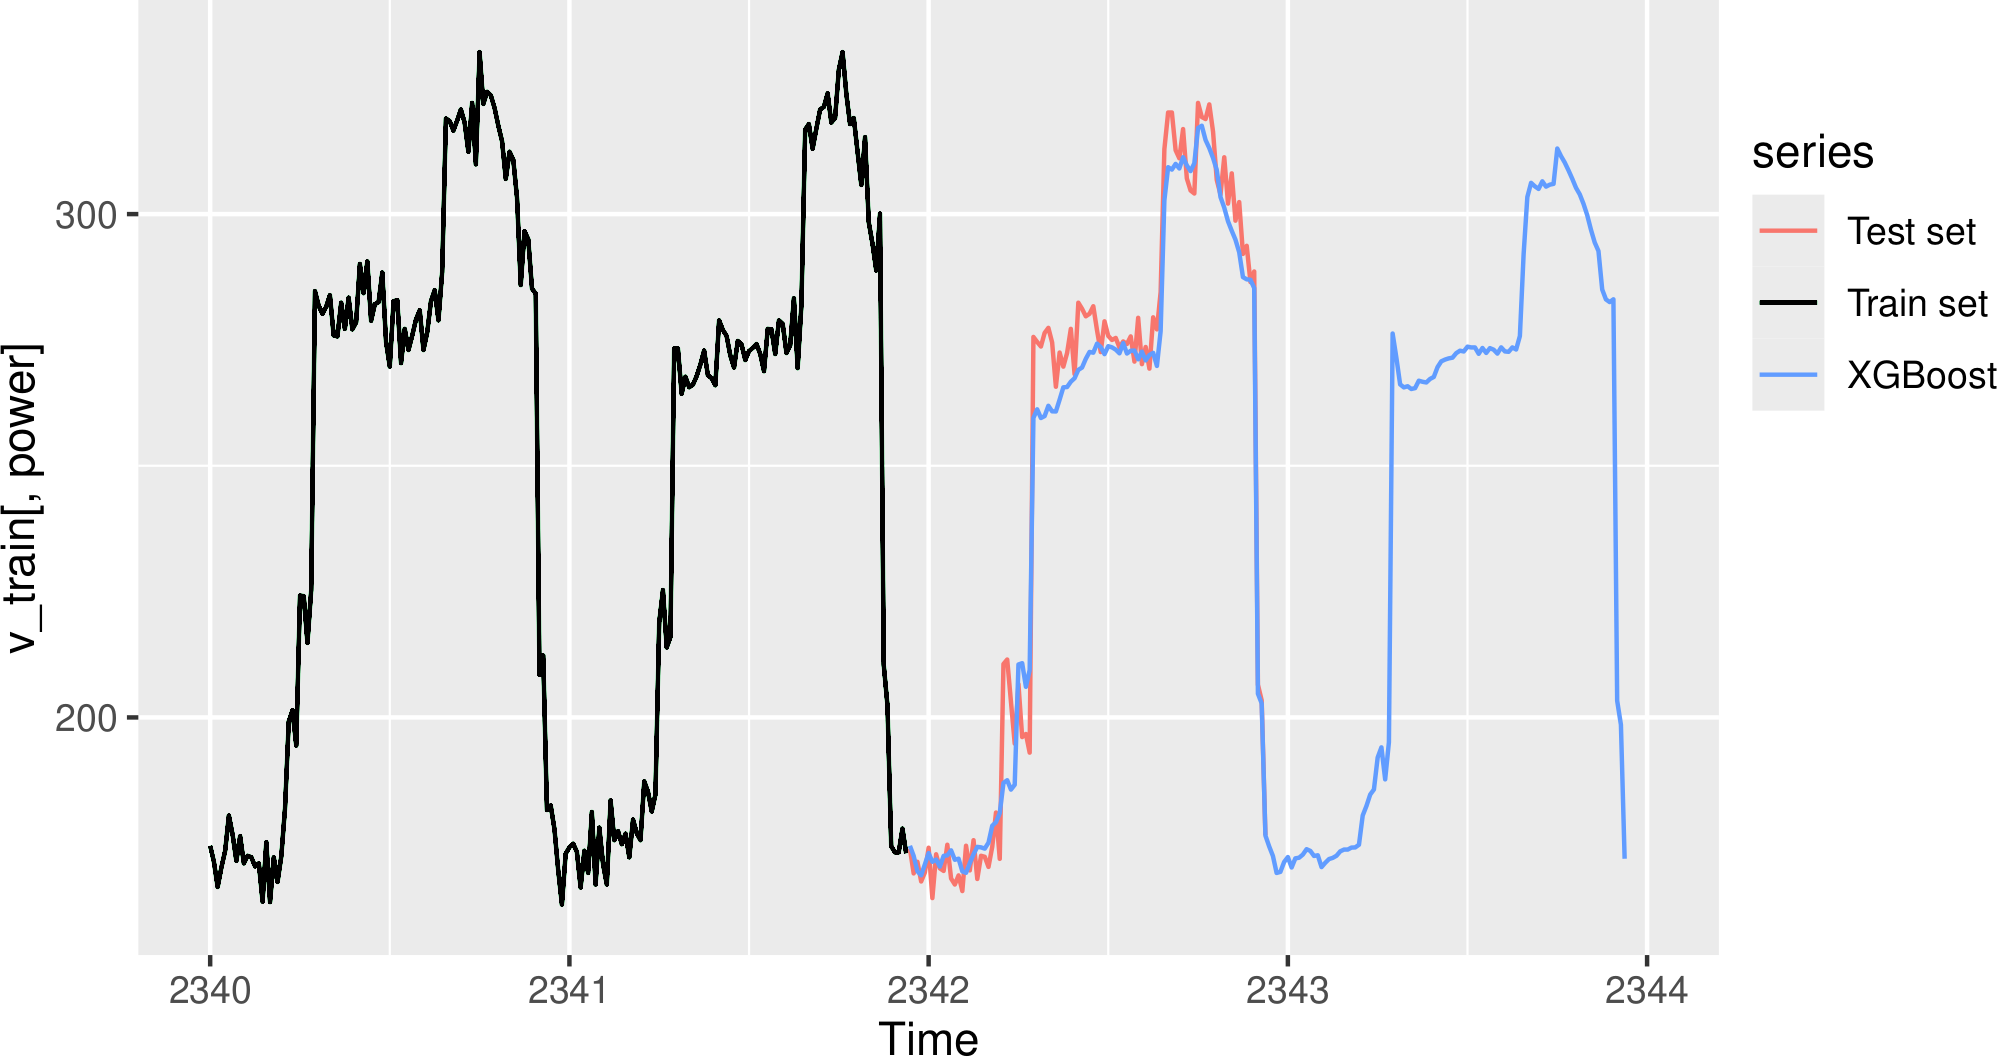
\includegraphics[scale=0.6]{figures/figure_xgboost.png}
\caption{Modelling and forecast using XGBoost algorithm without considering the OAT covariate.}
\label{figure_xgboost}
\end{figure}


